Describe here work that is connected to your thesis. This should include
references to published work. There is no fixed rule, but I would expect a
student to have read around 50 published research papers and reference them in a
thesis.

\section{Evaluation metrics}

For multiclass classification problems, e.g.\ identifying a sample as a
particular bird species from a last of $n > 2$ species, a simple classification
accuracy is often used as an evaluation metric
(\cite{chakraborty2016bird},~\cite{ramashini2022robust}). This is calculated as
the percentage of correctly identified samples from a set of labelled samples
previously unseen by the model.

Acevedo et al~\cite{acevedo2009automated} used true positive ($TP$) and false
positive ($FP$) rates to evaluate their models used to classify bird and amphibian
calls. This evaluation method is sometimes preferred when analysing long
recordings which may include several different species to be classified. $TP$
gives an indication as to how well the model correctly identifies species
present in the recording. $FP$ indicates how often the model erroneously
identifies species absent in the recording. A high performing model will have
high values for $TP$ and low values for $FP$\@.

Potamitis et al~\cite{potamitis2014automatic} used an alternative form of
evaluation presented in terms of precision $(P)$ and recall $(R)$ which are
defined as
\begin{equation}
  P = \frac{\text{TP}}{\text{TP}+\text{FP}}, \hspace{1em}
  R = \frac{\text{TP}}{\text{TP}+\text{FN}}
\end{equation}
where $FN$ is the number of false negatives. Informally, $P$ and $R$ can be
thought of as
\begin{equation}
  P = \frac{\text{relevant retrieved instances}}{\text{all \textbf{retrieved} instances}}, \hspace{1em}
  R = \frac{\text{relevant retrieved instances}}{\text{all \textbf{relevant} instances}}
\end{equation}
It's well known that there is usually a trade-off between $P$ and $R$, so
usually the $F$-score is reported along with the $P$ and $R$ metrics. The
$F$-score is defined as
\begin{equation}
F = \frac{(1+\beta^2)PR}{\beta^2P + R}
\end{equation}
for some $\beta \in \mathbb{R}$.

For binary classification problems, i.e.\ classifying a sample as one of two
classes (bird species), the Area Under Curve (AUC) metric is sometimes
preferred~\cite{leng2014multi}. The AUC ranges from 0 to 1, with a higher value
indicating a better performing model. The AUC is sometimes desirable because it
is scale-invariant (it measures how well predictions are ranked, rather than
their absolute values) and classification-threshold-invariant (it measures the
quality of the model's predictions regardless of what classification threshold
is chosen.)

\section{Feature extraction}

As mentioned in Chapter~\ref{cp:intro}, birds use vocalizations as a way to
communicate with others. Birds have evolved over many thousands of years to
make this form of communication very efficient in that it can travel long
distances and cut through local ambient noise frequencies so that it can be
received by other birds clearly. Some birds have even adapted their
vocalizations so that they can be heard in local environments that have rapidly
changed over the past decades, such as urban areas with increasing anthropogenic
noise~\cite{luther2010urban}.

Bird vocalizations can be broadly divided into two main categories, calls and
songs. Calls are typically short vocalizations that carry some specific
function, such as warning others to the presence of a predator or calling others
to flight~\cite{MARLER2004132}. Songs are usually longer and more acoustically
complex and occur more spontaneously. Songs are typically employed as breeding
calls or territorial defence. While all birds produce calls, in many species of
birds only the males utilise songs and often only during breeding season. The
song and call of a Eurasian Wren can be seen and contrasted in
figure~\ref{fig:wren_call_song_spectrogram}.

Doupe et al~\cite{birdsongspeech} showed that there were striking similarities
between birdsong and human language. Similar to human language, birdsong can be
thought of as comprised of hierarchical levels of phrases, syllables, and
elements~\cite{catchpole2003bird}. <Figure here>. Raw recordings of birdsong
often contain periods of silence that occur between phrases which are unlikely
to provide useful information in order to train a machine learning model.
Fagerlund~\cite{fagerlund2007bird} showed that a good level of accuracy can be
achieved by training models on features extracted from segmented syllables which
were used as training samples. An algorithm for robust syllable segmentation was
proposed in~\cite{fagerlund2004automatic} and is used in this thesis. The
algorithm is described in more detail in Section.

\begin{figure}[ht]
  \centering
  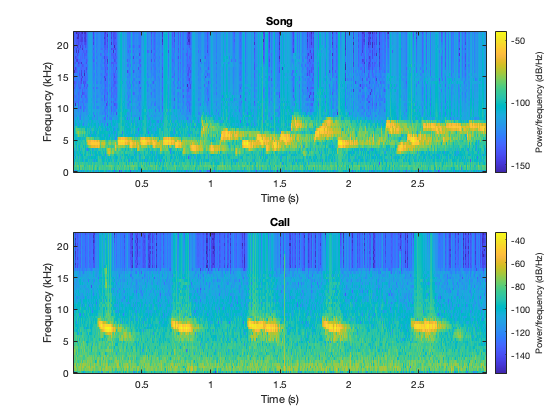
\includegraphics[width=\textwidth]{figures/wren_call_song_spectrogram.png}
  \caption{Spectrograms of the call and song of the Eurasian Wren
    (\textit{Troglodytes troglodytes}). As can be seen, the song is much more complex in terms of pitch and acoustic structure compared to the
  call}\label{fig:wren_call_song_spectrogram}
\end{figure}

Once the syllables have been segmented, there exists an abundance of options to
turn the raw syllable input signal into features that might be used as training
samples. In the following sections some of the more popular feature
representations are described, along with some novel methods that have yet to be
tried on birdsong. Note that the following list is certainly not exhaustive and
emphasis has been placed on feature representations that are relevant to this
thesis.

\subsection{Features inspired by the human auditory system}

Research has shown that birdsong and human language share many similarities in
terms of the neural mechanisms employed to form the language/song, the impact of
social contact in learning the language/song, and so on~\cite{birdsongspeech}.
Give that the human auditory system has evolved other thousands of years to best
process human speech, it seems reasonable to suggest that using features based
on the human auditory system may be effective when it comes to birdsong.

At a high level, the human auditory system works by translating changes in air
pressure originating from a source and reaching the outer ear of a listener
into vibrations that travel along an internal organ known as a cochlear. The
vibrations trigger electric signals that move along auditory nerves to the
brain, where they are interpreted as sounds. The physiology of the cochlear
means that certain parts of the organ are more sensitive to certain frequencies
of vibrations, so different frequencies will lead to different electrical
signals moving to the brain. This allows the brain to learn to differentiate
between frequencies.

\subsubsection{Mel frequency cepstrum coefficients}

The makeup of the human auditory system means that humans have a greater ability
to differentiate pitch at lower frequencies then they do at higher frequencies.
In other words, humans perceive pitch non-linearly. This has led to the
development of a logarithmic scale, known as the mel scale, such that equal
distances on the scale have the same \textit{perceptual} distance.

The mel frequency cepstrum coefficients (MFCC) are part of a family of cepstrum
coefficients that capture information about the rate of change in different
spectrum bands. MFCC differs from other cepstrum coefficients in that it uses the
mel scale to transform the spectrum of an input signal, thus utilising the human
auditory system in the calculation of its coefficients.

The $i$-th mel cepstral coefficient is computed as~\cite{davis1980comparison}
\begin{equation}
\text{MFCC}_i = \sum_{k=1}^{K} X_k \cos \left(
  \frac{i(k-0.5)\pi}{K}
\right)
\end{equation}
where $X_k$ is the logarithmic energy of the $k$-th mel-spectrum band, and $K$
is the total number of the mel-spectrum bands. Usually 8--13 MFCC coefficients
are used as the feature vector representing one time frame of the signal. The
0$^{th}$ coefficient is often excluded as it represents the average log energy
of the signal and is unlikely to carry any relevant information to help with
classification.

MFCCs are often presented with their delta ($\Delta$) and double-delta
($\Delta\Delta$) values that capture the local temporal dynamics and temporal
changes of the delta values respectively.

MFCCs are used as feature representations since they are simple to compute and
have been shown to have good performance in a wide range of audio classification
tasks, such as speaker identification~\cite{muda2010voice} and emotion
recognition~\cite{likitha2017speech}. MFCCs have also been shown to lead to good
classification accuracy for birdsong identification problems
(\cite{fagerlund2007bird} and~\cite{ramashini2022robust}).

<include graph of filterbank>

\subsubsection{Gammatone cepstrum coefficients}

Gammatone cepstrum coefficients (GTCCs) are similar to MFCCs except their
calculation  uses gammatone filterbanks instead of mel scale filterbanks.
Gammatone filterbanks are designed to simulate the motion of the membrane inside
the cochlear, known as the basilar membrane, when it is exposed to vibrations
transmitted by the outer and middle ear~\cite{patterson1992complex}.

A gammatone filter with a centre frequency $f_c$ is defined as
\begin{equation}
  g(t) = at^{n-1}e^{-2\pi b t} \cos(2\pi f_c + \psi)
\end{equation}
where $t$ is the time in seconds, $\psi$ is the phase in radians (usually set to
0), $a \in \mathbb{R}$ controls the gain, $n$ is the filter's order and $b$ is
the filter's bandwidth in Hz.

Similar to MFCCs, GTCCs are typically used with their $\Delta$ and $\Delta\Delta$
values and have also been shown to have a good performance in
non-speech audio classification problems~\cite{valero2012gammatone}.

<include graph of filterbank>

\subsubsection{Multi resolution cochleagram}

\subsection{Feature stacking}

\section{Classification}

\subsection{KNN}

KNN used by~\cite{ramashini2019bird}

\subsection{Decision trees}

Description of decision trees. Used by~\cite{acevedo2009automated}.

\subsection{Gaussian Mixture Models}

\subsection{Hidden Markov Models}

\subsection{SVMs}

\subsection{Neural Networks}

\subsubsection{Feedforward Neural Network}

\subsubsection{Convolutional Neural Network}

\subsubsection{Recurrent Neural Network}
